\documentclass{article}
\usepackage[utf8]{inputenc}
\usepackage{amsmath}
\usepackage{graphicx}
\usepackage{hyperref}
\usepackage{microtype}
\usepackage[section]{placeins}
\usepackage{booktabs}
\usepackage{float}
\usepackage[toc,title]{appendix}
\usepackage{listings}
\usepackage{color}
\definecolor{codegreen}{rgb}{0,0.6,0}
\definecolor{codegray}{rgb}{0.5,0.5,0.5}
\definecolor{codepurple}{rgb}{0.58,0,0.82}
\definecolor{backcolour}{rgb}{0.95,0.95,0.92}
\lstdefinestyle{mystyle}{
  backgroundcolor=\color{backcolour},
  commentstyle=\color{codegreen},
  keywordstyle=\color{magenta},
  numberstyle=\tiny\color{codegray},
  stringstyle=\color{codepurple},
  basicstyle=\ttfamily\footnotesize,
  breakatwhitespace=false,
  breaklines=true,
  captionpos=b,
  keepspaces=true,
  numbers=left,
  numbersep=5pt,
  showspaces=false,
  showstringspaces=false,
  showtabs=false,
  tabsize=2
}
\lstset{style=mystyle}
\title{543 Readmissions Project Exploratory Data Analysis Report}
\author{Jack Phelan}
\date{May 2026}
\begin{document}
\maketitle
\tableofcontents
\newpage

\section{Dataset Overview}
% Describe the source, size, and structure of the dataset.
% Include: number of records, number of features, target variable definition.
% Dataset source, number of records (rows) and variables (columns), file format, any metadata or documentation available
\par The dataset comes from two CSV files, \texttt{healthcare\_readmissions\_dataset\_train} and \texttt{healthcare\_readmissions\_dataset\_test}, each row consisting of one patient encounter. The training file contains 8,038 rows and 19 columns (including the target variable).

\begin{figure}[h]
  \centering
  
\includegraphics[width=\textwidth]{data_dictionary.png}
  \caption{Data Dictionary}
  \label{fig:data_dictionary}
\end{figure}

\noindent It is worth noting that \texttt{Has Chronic Kidney Disease},  \texttt{Post-Discharge Satisfaction Score}, and \texttt{Living Situation}
are not actually present in the files, despite being in the dictionary.

\section{Data Quality Summary}
% Summarize missing values, duplicates, and any data integrity issues found.
% Include a table of missing value counts/percentages per feature.
% Summarize the quality and completeness of the raw data
% Identify unusual data points or distributions (outliers)
\par Only two features in the dataset have missing values: \texttt{Number of Prior Visits} (314 rows or 3.9\%) and
\texttt{Medications Prescribed} (657 rows or 8.2\%). The remaining features are complete, with no duplicates in the training set either.
Although boolean columns are not consistent in datatype (\texttt{Smoker} is a boolean column while \texttt{Has Diabetes} and \texttt{Has Hypertension} are integers with values of 0 and 1),
this can be handled quite easily during preprocessing.

\par \texttt{Exercise Frequency} and \texttt{Type of Treatment} also feature 'None' as a possible value,
which the \texttt{pandas} function \texttt{pd.read\_csv()} will interpret as a \texttt{NaN} by default. Again, this is not a major issue,
just something to be aware of.

\par A glance at the distribution of variables shows that \texttt{Age} has problematic outliers, in the form of patients over the age of
100.

\begin{figure}[H]
  \centering
  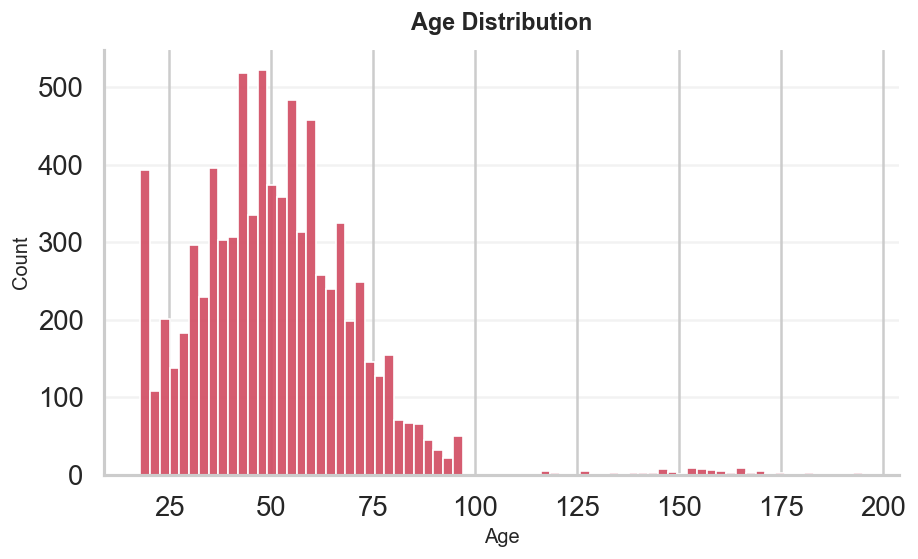
\includegraphics[width=\textwidth]{raw_df_age_histogram.png}
  \caption{Raw Age Distribution}
  \label{fig:age_histogram}
\end{figure}

\FloatBarrier
\par Using z-scores to identify outliers (as well as common sense), 80 rows were determined to be outliers and subsequently removed from the dataset.
These rows make up 0.99\% of the training set; although I would prefer to keep as much data as possible, these rows are clearly unrepresentative of real patients (for whatever reason),
and could potentially skew the results of any analysis or modeling.

\section{Statistical Summary}
% Provide descriptive statistics for numeric features (mean, median, std, min, max).
% Summarize categorical feature cardinalities.
% Summary statistics for measures (mean, median, std dev) and frequency distributions (counts) for categories

\par All stats are derived from the training set with the age outliers removed as outlined
in the previous section.

\begin{samepage}
  \subsection{Numeric Statistics}

  \begin{table}[H]
    \caption{Measure Summary Statistics}
    \label{tab:metrics}
    \resizebox{\textwidth}{!}{%
      \begin{tabular}{lrrrrrrrr}
        \toprule
        & count & mean & std & min & 25\% & 50\% & 75\% & max \\
        \midrule
        age & 7958.000000 & 50.110000 & 17.300000 & 18.000000 & 38.000000 & 50.000000 & 62.000000 & 95.000000 \\
        height\_m & 7958.000000 & 1.700000 & 0.100000 & 1.300000 & 1.600000 & 1.700000 & 1.800000 & 2.000000 \\
        bmi & 7958.000000 & 26.260000 & 4.750000 & 8.300000 & 23.100000 & 26.200000 & 29.300000 & 44.000000 \\
        weight\_kg & 7958.000000 & 77.150000 & 18.950000 & 23.300000 & 64.800000 & 75.400000 & 87.300000 & 236.300000 \\
        adjusted\_weight\_kg & 7958.000000 & 76.270000 & 16.660000 & 23.130000 & 64.730000 & 75.130000 & 86.860000 & 159.050000 \\
        has\_diabetes & 7958.000000 & 0.130000 & 0.340000 & 0.000000 & 0.000000 & 0.000000 & 0.000000 & 1.000000 \\
        has\_hypertension & 7958.000000 & 0.170000 & 0.380000 & 0.000000 & 0.000000 & 0.000000 & 0.000000 & 1.000000 \\
        number\_of\_prior\_visits & 7646.000000 & 3.040000 & 1.740000 & 0.000000 & 2.000000 & 3.000000 & 4.000000 & 11.000000 \\
        medications\_prescribed & 7308.000000 & 3.510000 & 1.960000 & 0.000000 & 2.000000 & 3.000000 & 5.000000 & 12.000000 \\
        length\_of\_stay & 7958.000000 & 2.540000 & 2.970000 & 0.000000 & 0.000000 & 2.000000 & 4.000000 & 23.000000 \\
        readmission\_within\_30\_days & 7958.000000 & 0.170000 & 0.380000 & 0.000000 & 0.000000 & 0.000000 & 0.000000 & 1.000000 \\
        \bottomrule
      \end{tabular}%
    }
  \end{table}

  \subsection{Categorical Statistics}

  \begin{figure}[H]
    \centering
    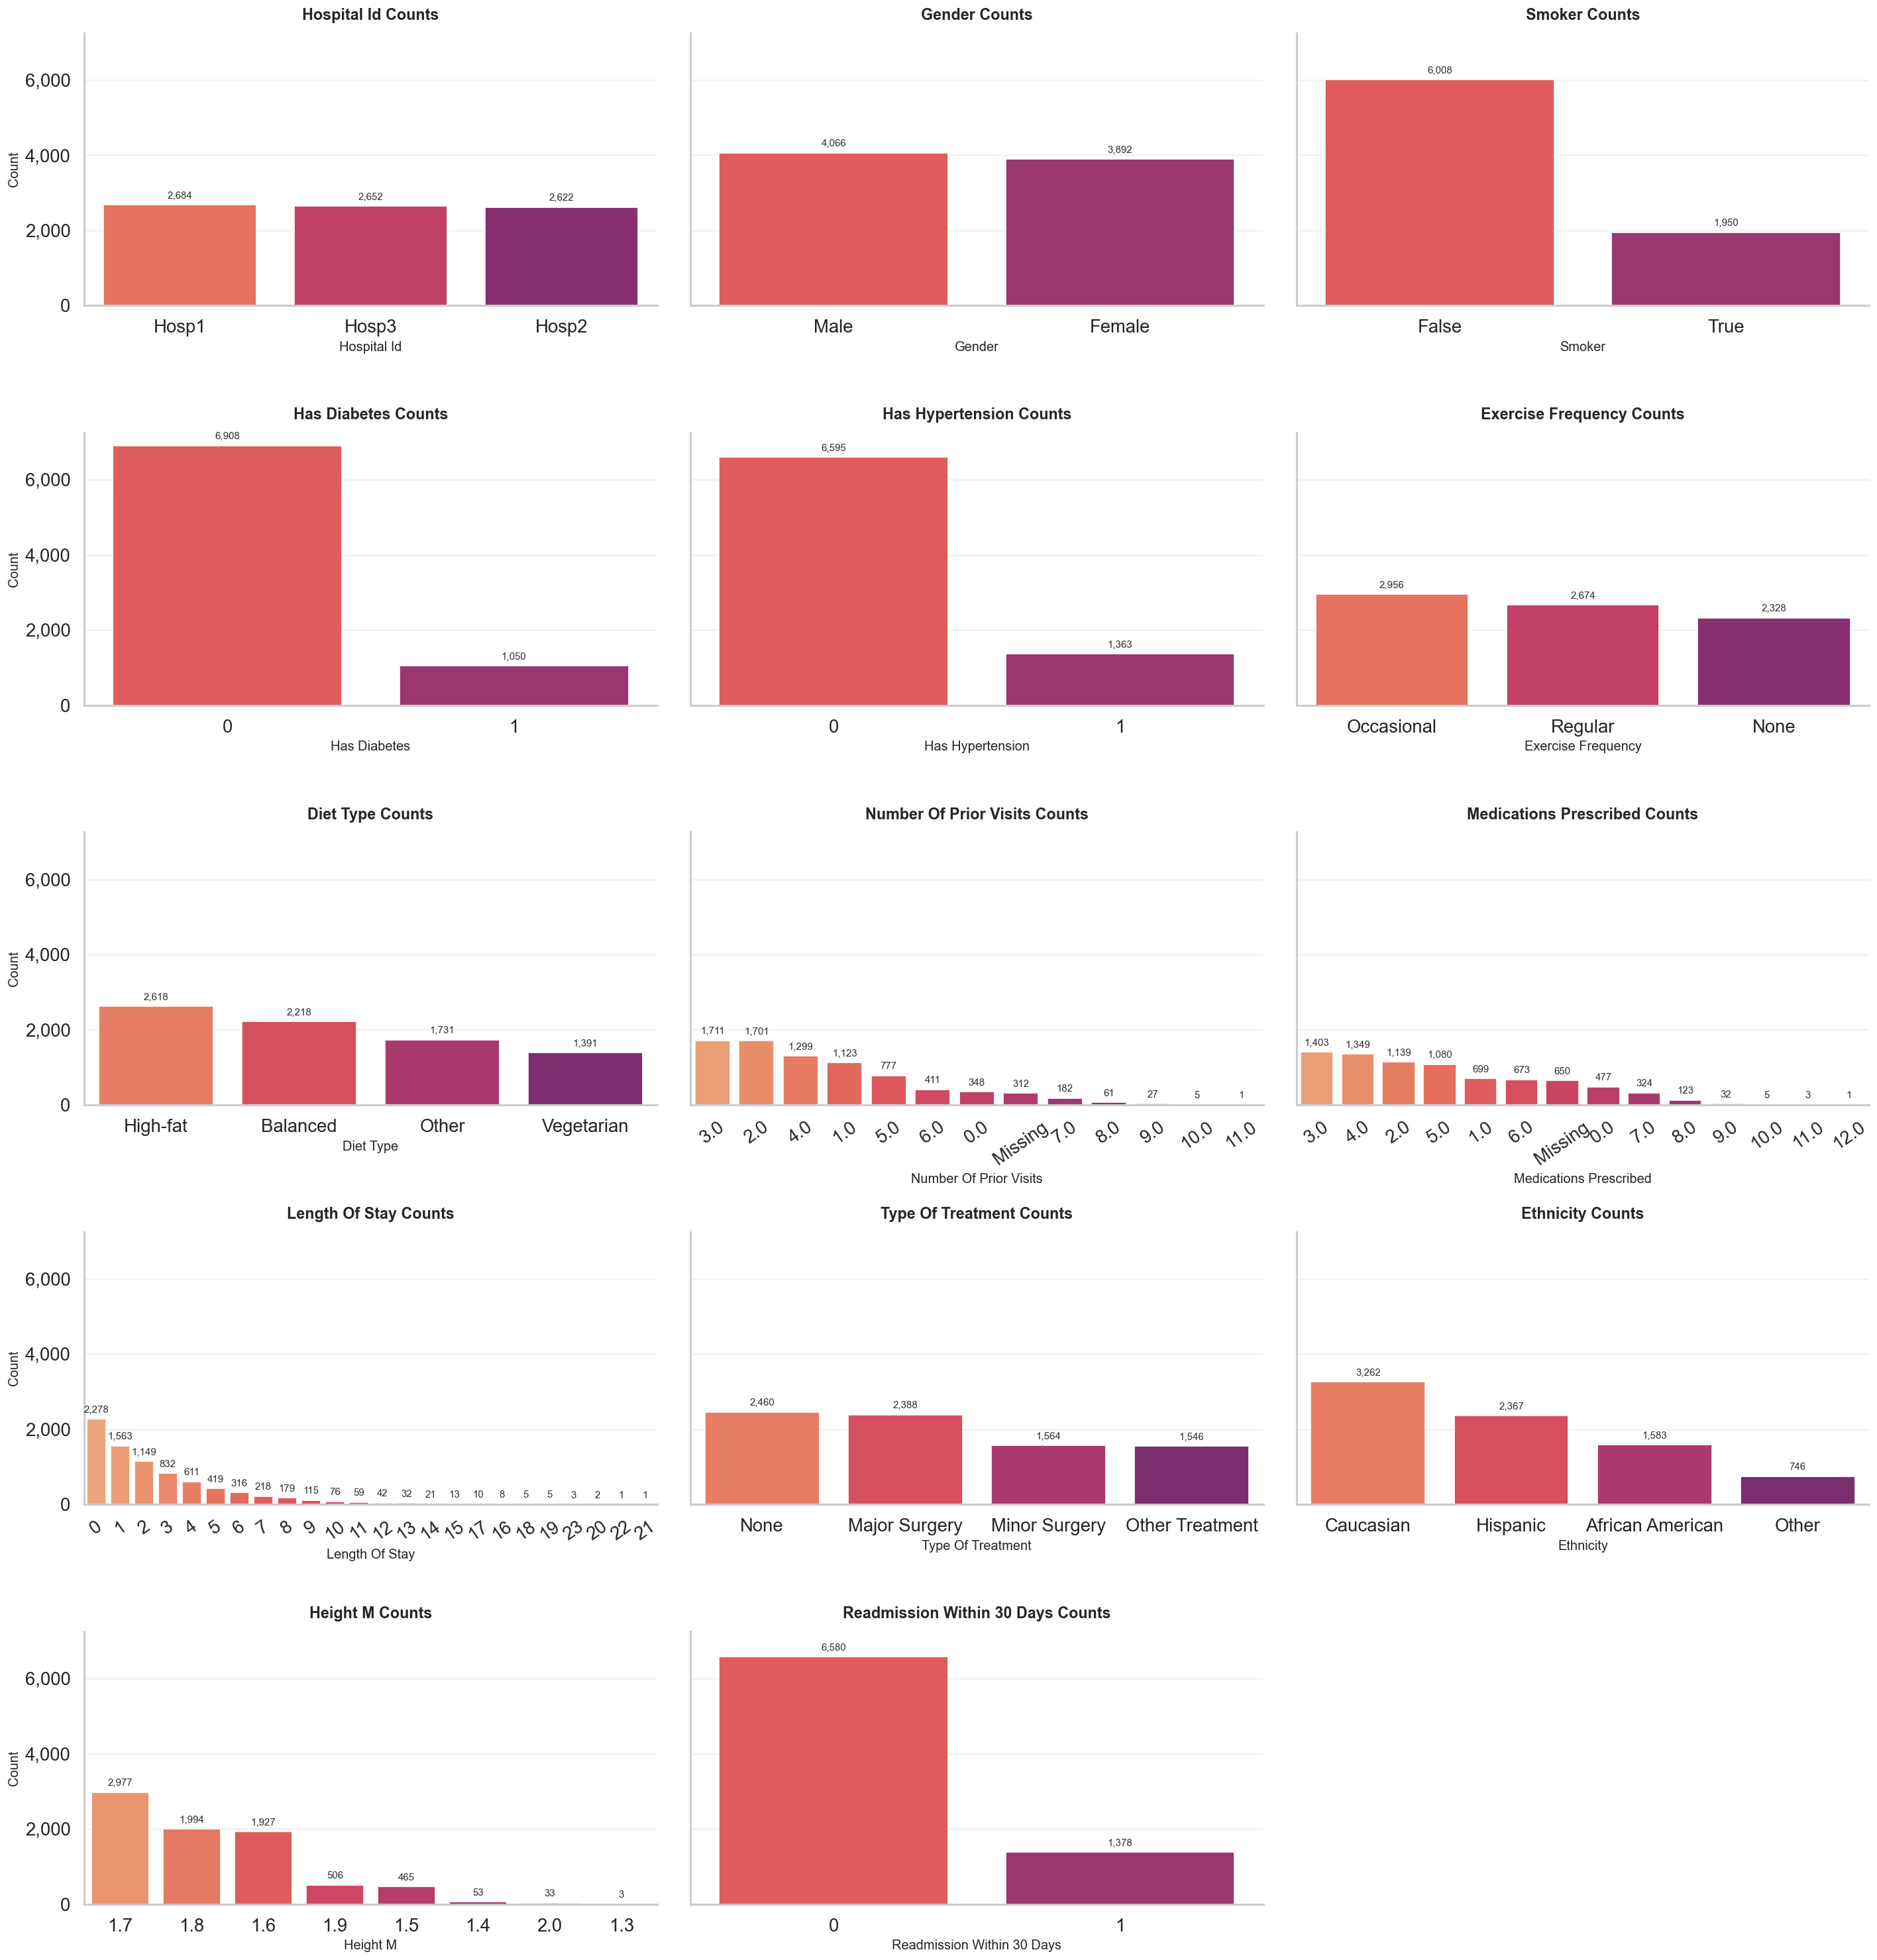
\includegraphics[width=0.7\textwidth]{category_distributions.png}
    \caption{Category Distributions}
    \label{fig:category_distributions}
  \end{figure}

  Individual distributions can be found in the \textbf{\nameref{sec:univariate-analysis}} section below.

\end{samepage}

\section{Univariate Analysis}
\label{sec:univariate-analysis}
% Analyze the distribution of each feature individually.
% Include histograms/bar charts and note any skew, outliers, or imbalance.

\subsection{Numeric Features}

\begin{figure}[H]
  \centering
  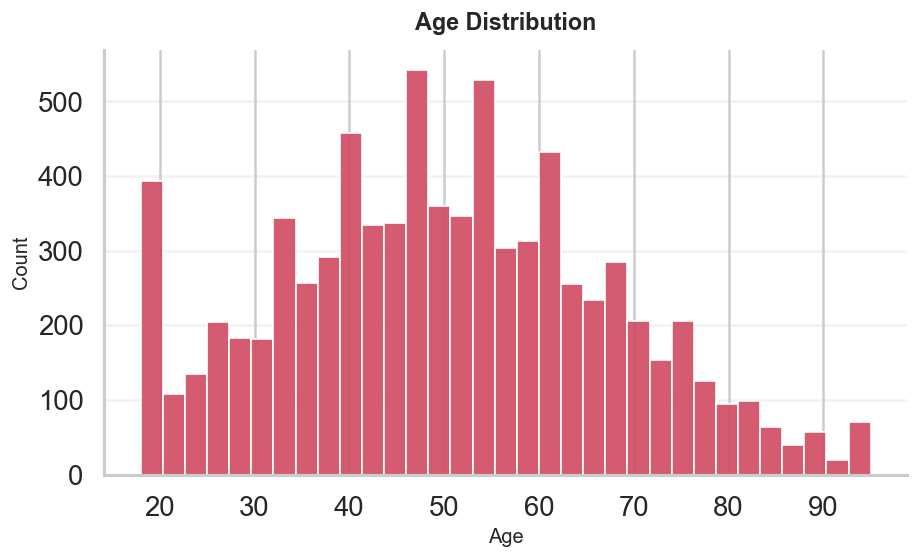
\includegraphics[width=0.75\textwidth]{age_dist.png}
  \caption{Age Histogram}
  \label{fig:age_dist}
\end{figure}

The distribution with removed outliers makes much more sense compared to the raw values.

\begin{figure}[H]
  \centering
  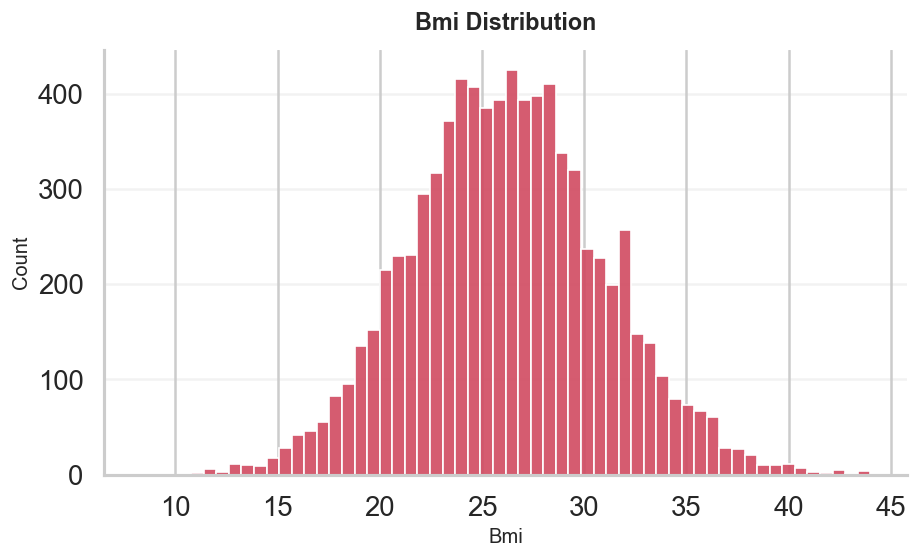
\includegraphics[width=0.75\textwidth]{bmi_hist.png}
  \caption{BMI Histogram}
  \label{fig:bmi_dist}
\end{figure}

For the most part normal; some values on the ends are in the extreme but not necessarily impossible
(e.g.\ a BMI of 44 is very high but not unheard of).

\begin{figure}[H]
  \centering
  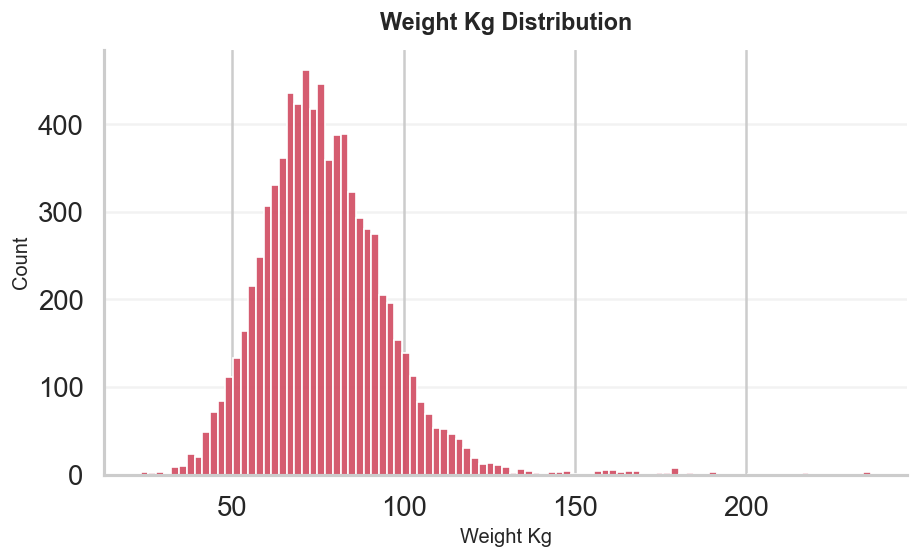
\includegraphics[width=0.75\textwidth]{weight_hist.png}
  \caption{Weight Histogram}
  \label{fig:weight_dist}
\end{figure}

Similar to BMI, some extreme values but nothing that stands out as impossible. Also makes
sense that its similar to BMI as they are highly correlated.

\begin{figure}[H]
  \centering
  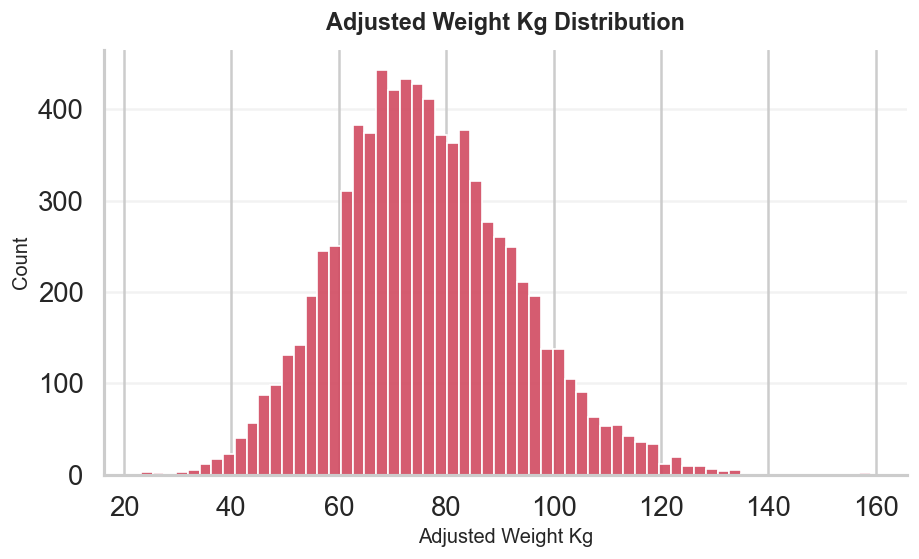
\includegraphics[width=0.75\textwidth]{adj_weight_hist.png}
  \caption{Adjusted Weight Histogram}
  \label{fig:adj_weight_dist}
\end{figure}

Less outliers than standard weight, however the \nameref{fig:data_dictionary} does not specify how (or why) its adjusted,
so it's hard to make any judgments or comparisons to standard weight.

\subsection{Categorical Features}
\begin{figure}[H]
  \centering
  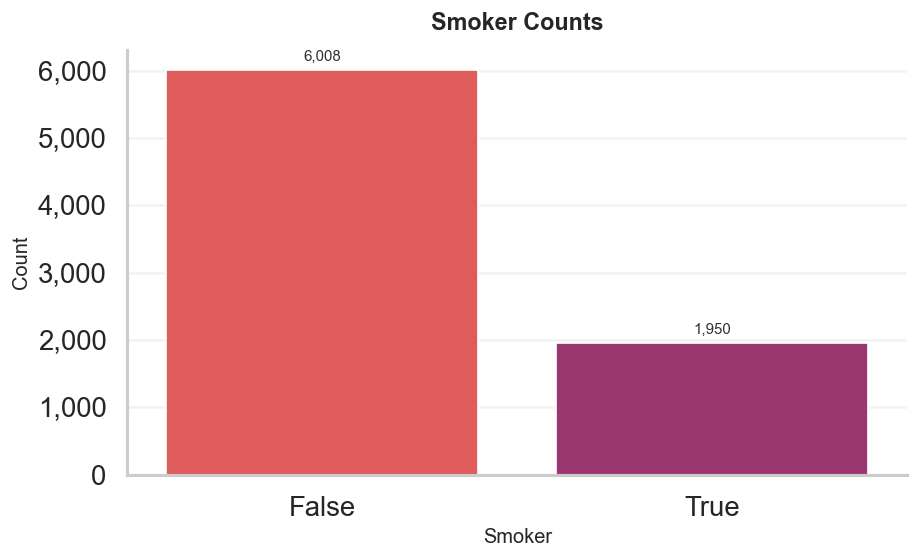
\includegraphics[width=0.75\textwidth]{smoker_bar.png}
  \caption{Smoker Bar Chart}
  \label{fig:smoker_bar}
\end{figure}

\begin{figure}[H]
  \centering
  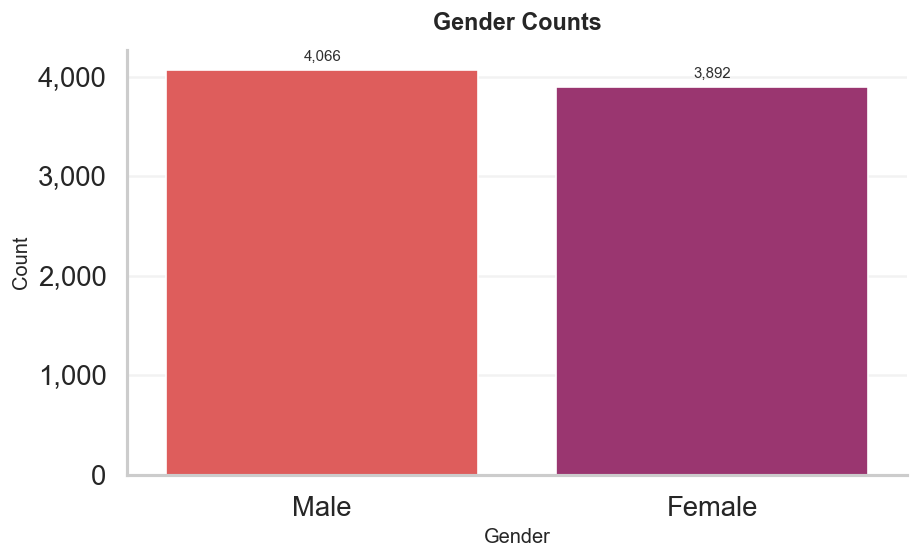
\includegraphics[width=0.75\textwidth]{gender_bar.png}
  \caption{Gender Bar Chart}
  \label{fig:gender_bar}
\end{figure}

\begin{figure}[H]
  \centering
  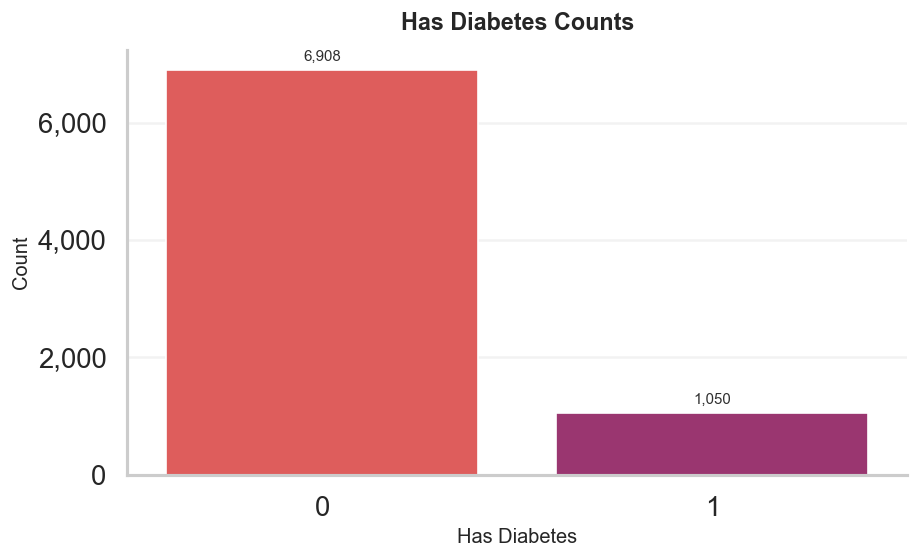
\includegraphics[width=0.75\textwidth]{diabetes_bar.png}
  \caption{Diabetes Bar Chart}
  \label{fig:diabetes_bar}
\end{figure}

\begin{figure}[H]
  \centering
  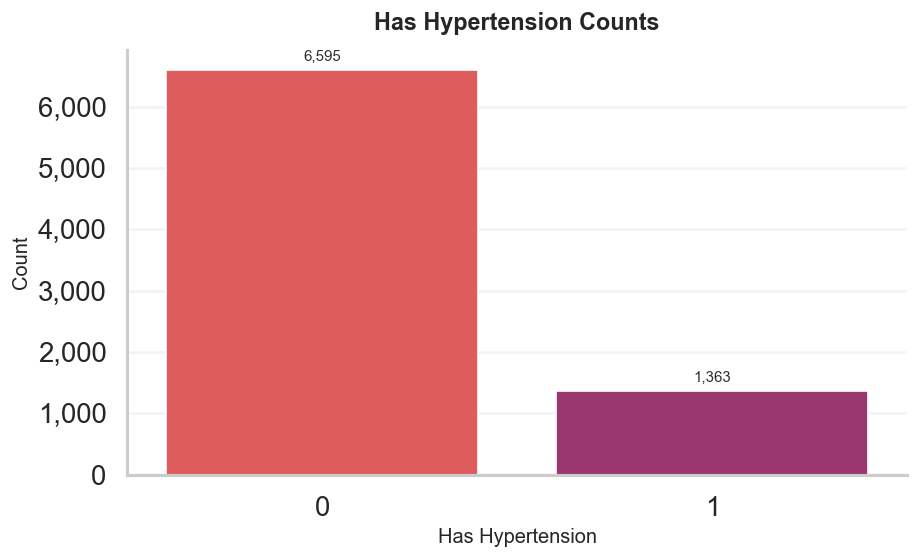
\includegraphics[width=0.75\textwidth]{hypertension_bar.png}
  \caption{Hypertension Bar Chart}
  \label{fig:hypertension_bar}
\end{figure}

\begin{figure}[H]
  \centering
  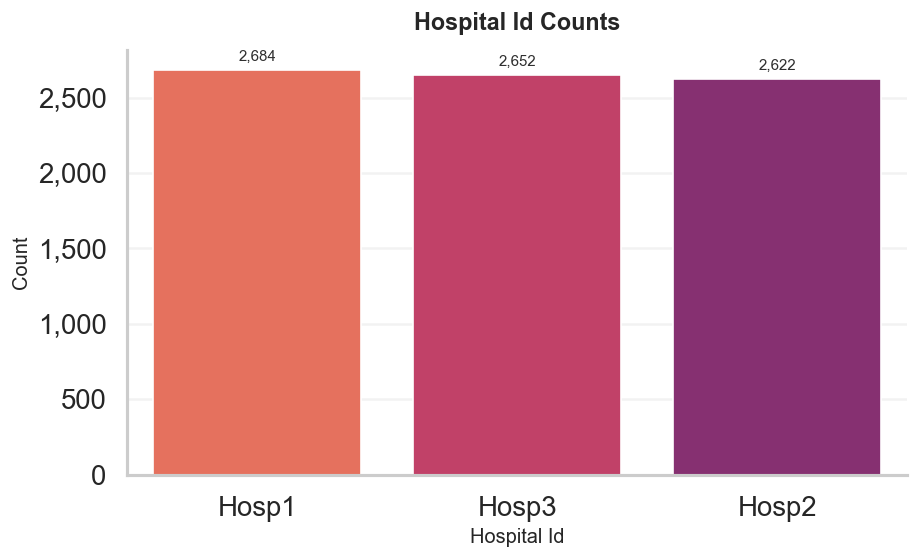
\includegraphics[width=0.75\textwidth]{hospital_id_bar.png}
  \caption{Hospital ID Bar Chart}
  \label{fig:hospital_id_bar}
\end{figure}

\begin{figure}[H]
  \centering
  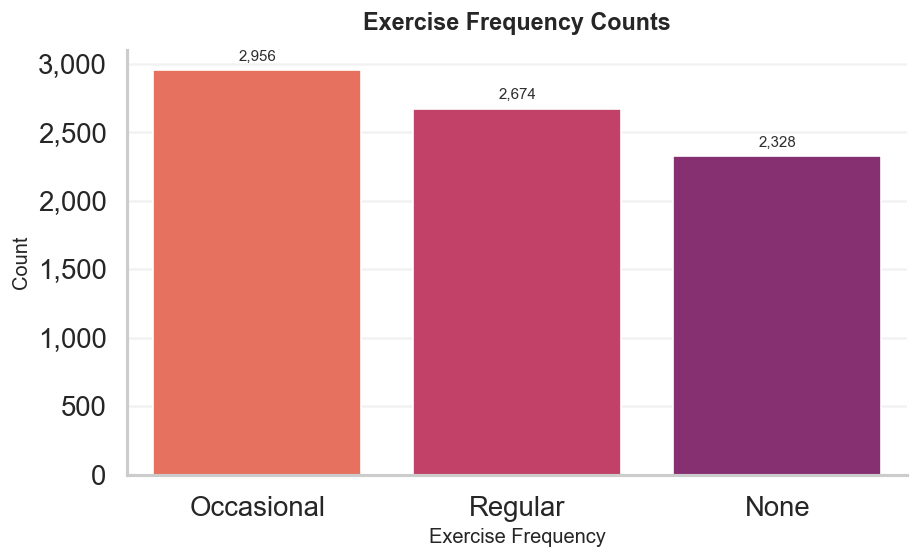
\includegraphics[width=0.75\textwidth]{excercise_freq_bar.png}
  \caption{Exercise Frequency Bar Chart}
  \label{fig:excercise_freq_bar}
\end{figure}

\begin{figure}[H]
  \centering
  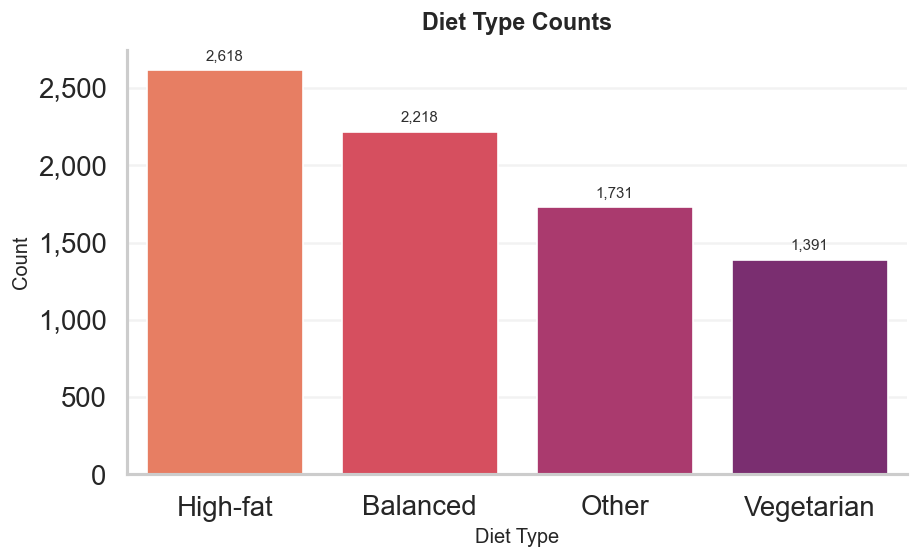
\includegraphics[width=0.75\textwidth]{diet_bar.png}
  \caption{Diet Bar Chart}
  \label{fig:diet_bar}
\end{figure}

\begin{figure}[H]
  \centering
  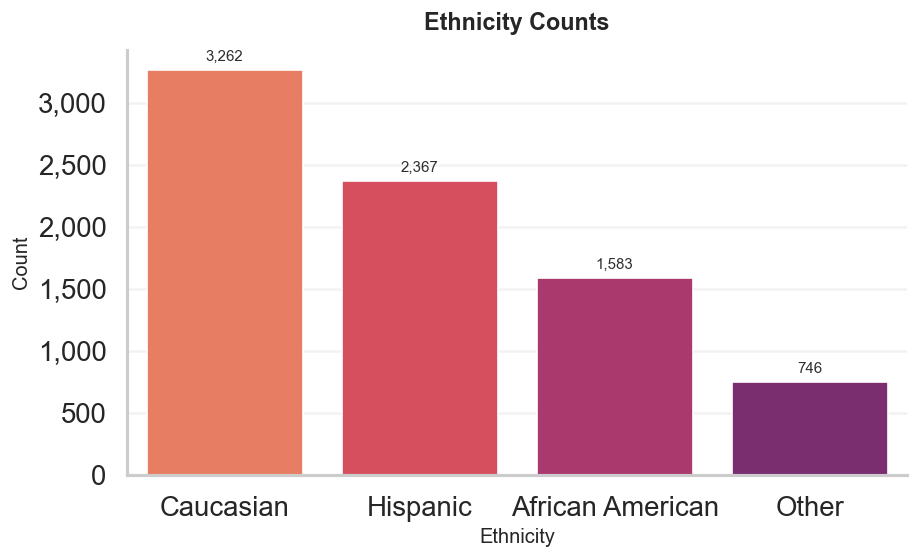
\includegraphics[width=0.75\textwidth]{ethnicity_bar.png}
  \caption{Ethnicity Bar Chart}
  \label{fig:ethnicity_bar}
\end{figure}

Figures 8 through 15 are all quite unremarkable and to be expected for the dataset.

\begin{figure}[H]
  \centering
  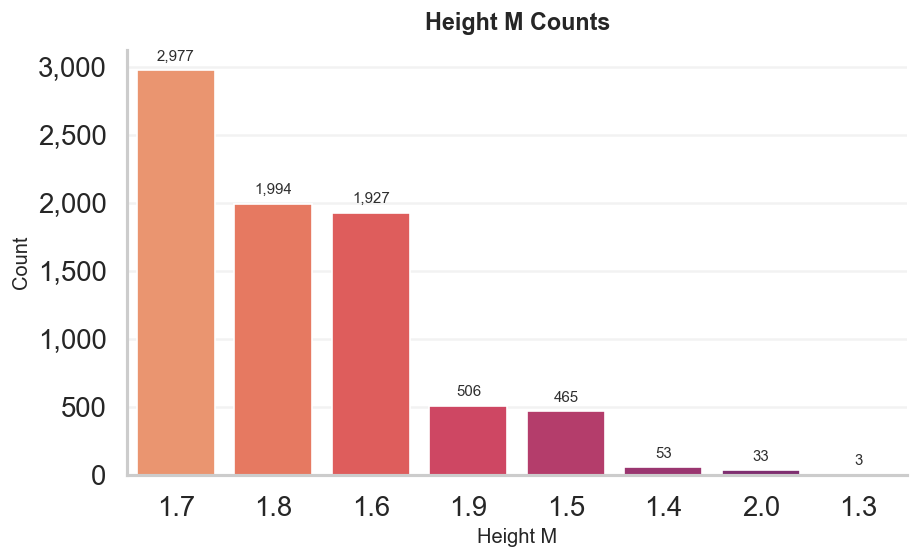
\includegraphics[width=0.75\textwidth]{height_bar.png}
  \caption{Height Bar Chart}
  \label{fig:height_bar}
\end{figure}

Also expected, although interesting that the height is stored in what is essentially categorical form,
rather than more precise measurements.

\begin{figure}[H]
  \centering
  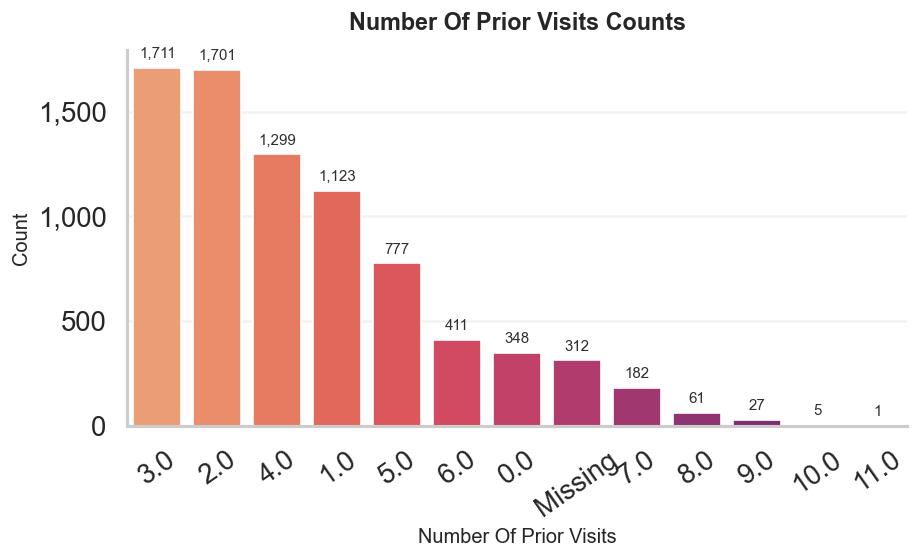
\includegraphics[width=0.75\textwidth]{prior_vis_bar.png}
  \caption{Prior Visits Bar Chart}
  \label{fig:prior_vis_bar}
\end{figure}

Has a very long tail, and also missing values are quite prevalent. Would potentially make sense
to group/encode values somehow, but that will be looked into during modeling and feature engineering.

\begin{figure}[H]
  \centering
  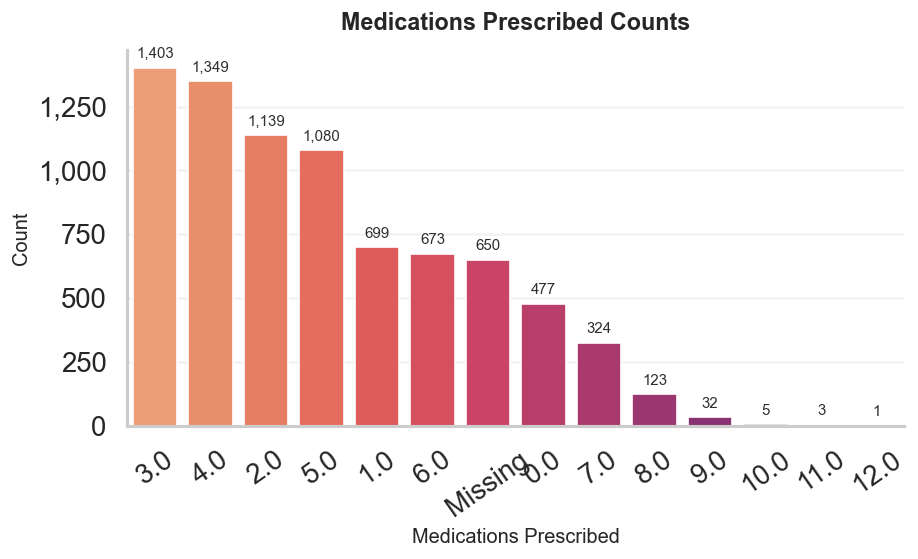
\includegraphics[width=0.75\textwidth]{meds_presc_bar.png}
  \caption{Medications Prescribed Bar Chart}
  \label{fig:meds_presc_bar}
\end{figure}

A somewhat similar situation to prior visits, although an overall smaller range of values.
Maybe worth grouping into ranges, or just full binary of 0 vs.\ 1 or more prescriptions.

\begin{figure}[H]
  \centering
  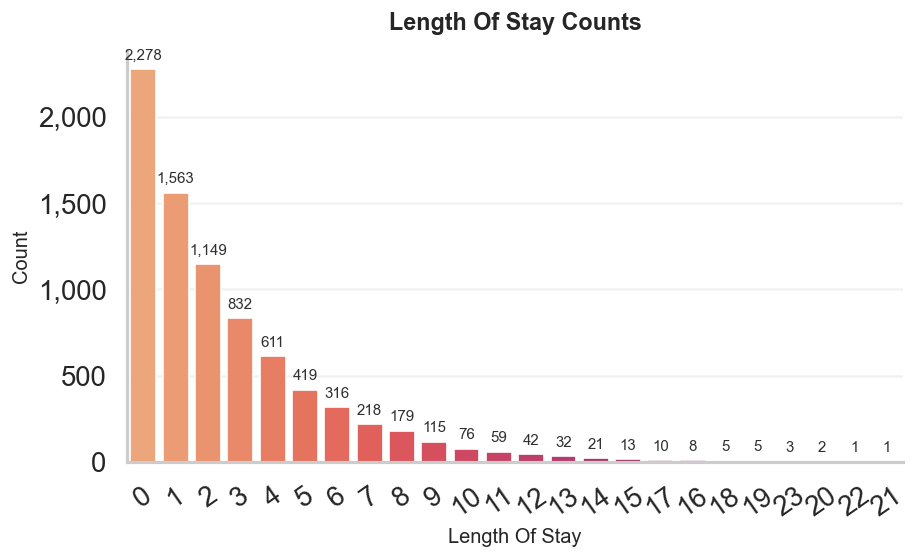
\includegraphics[width=0.75\textwidth]{los_bar.png}
  \caption{Length of Stay Bar Chart}
  \label{fig:los_bar}
\end{figure}
Long tail, no missing values. Should be encoded somehow, should look to common techniques
other projects/models have used in the past as it seems like a common and important feature in healthcare datasets.

\begin{figure}[H]
  \centering
  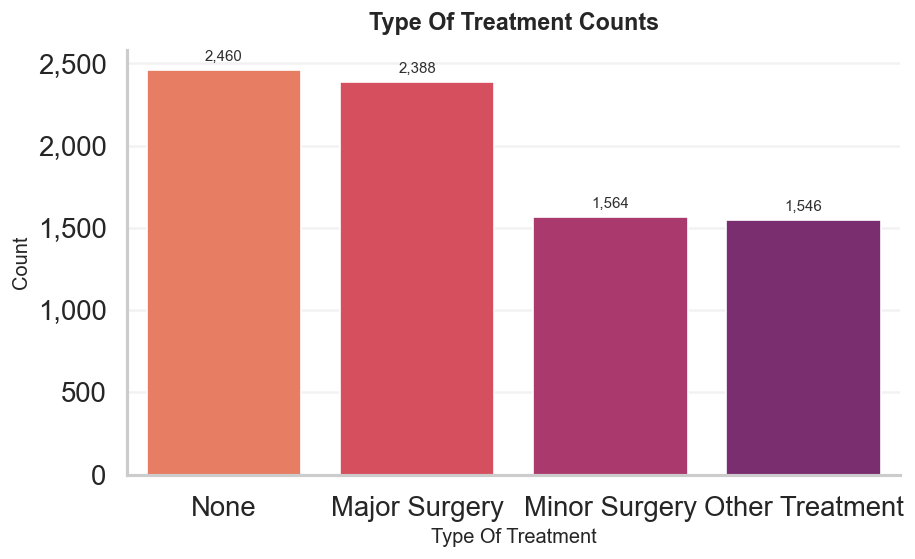
\includegraphics[width=0.75\textwidth]{treatment_type_bar.png}
  \caption{Treatment Type Bar Chart}
  \label{fig:treatment_type_bar}
\end{figure}

Somewhat vague categories, more experimentation on encoding strategies should be revealing as per best utilizing the feature.

\begin{figure}[H]
  \centering
  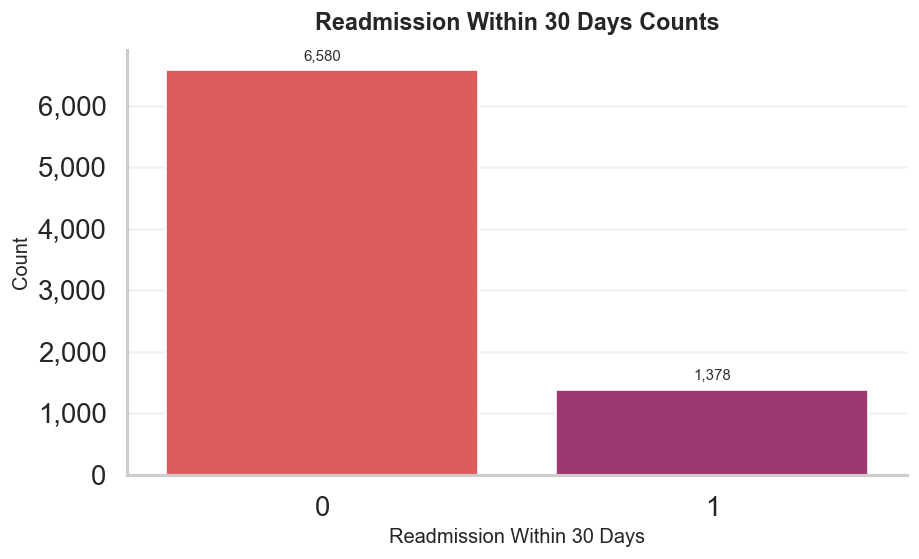
\includegraphics[width=0.75\textwidth]{read_bar.png}
  \caption{Readmission (Target) Bar Chart}
  \label{fig:read_bar}
\end{figure}

Output variable. Very skewed, should consider that in model selection and/or resambling techniques.

\section{Bivariate Analysis}
% Bivariate visualizations of each variable vs the response variable and any other “interesting” pairs of variables.
% Can be done with Tableau or Python
% Annotate any significant observations

\subsection{Feature vs.\ Target}

\subsubsection{Categories}
\begin{figure}[H]
  \centering
  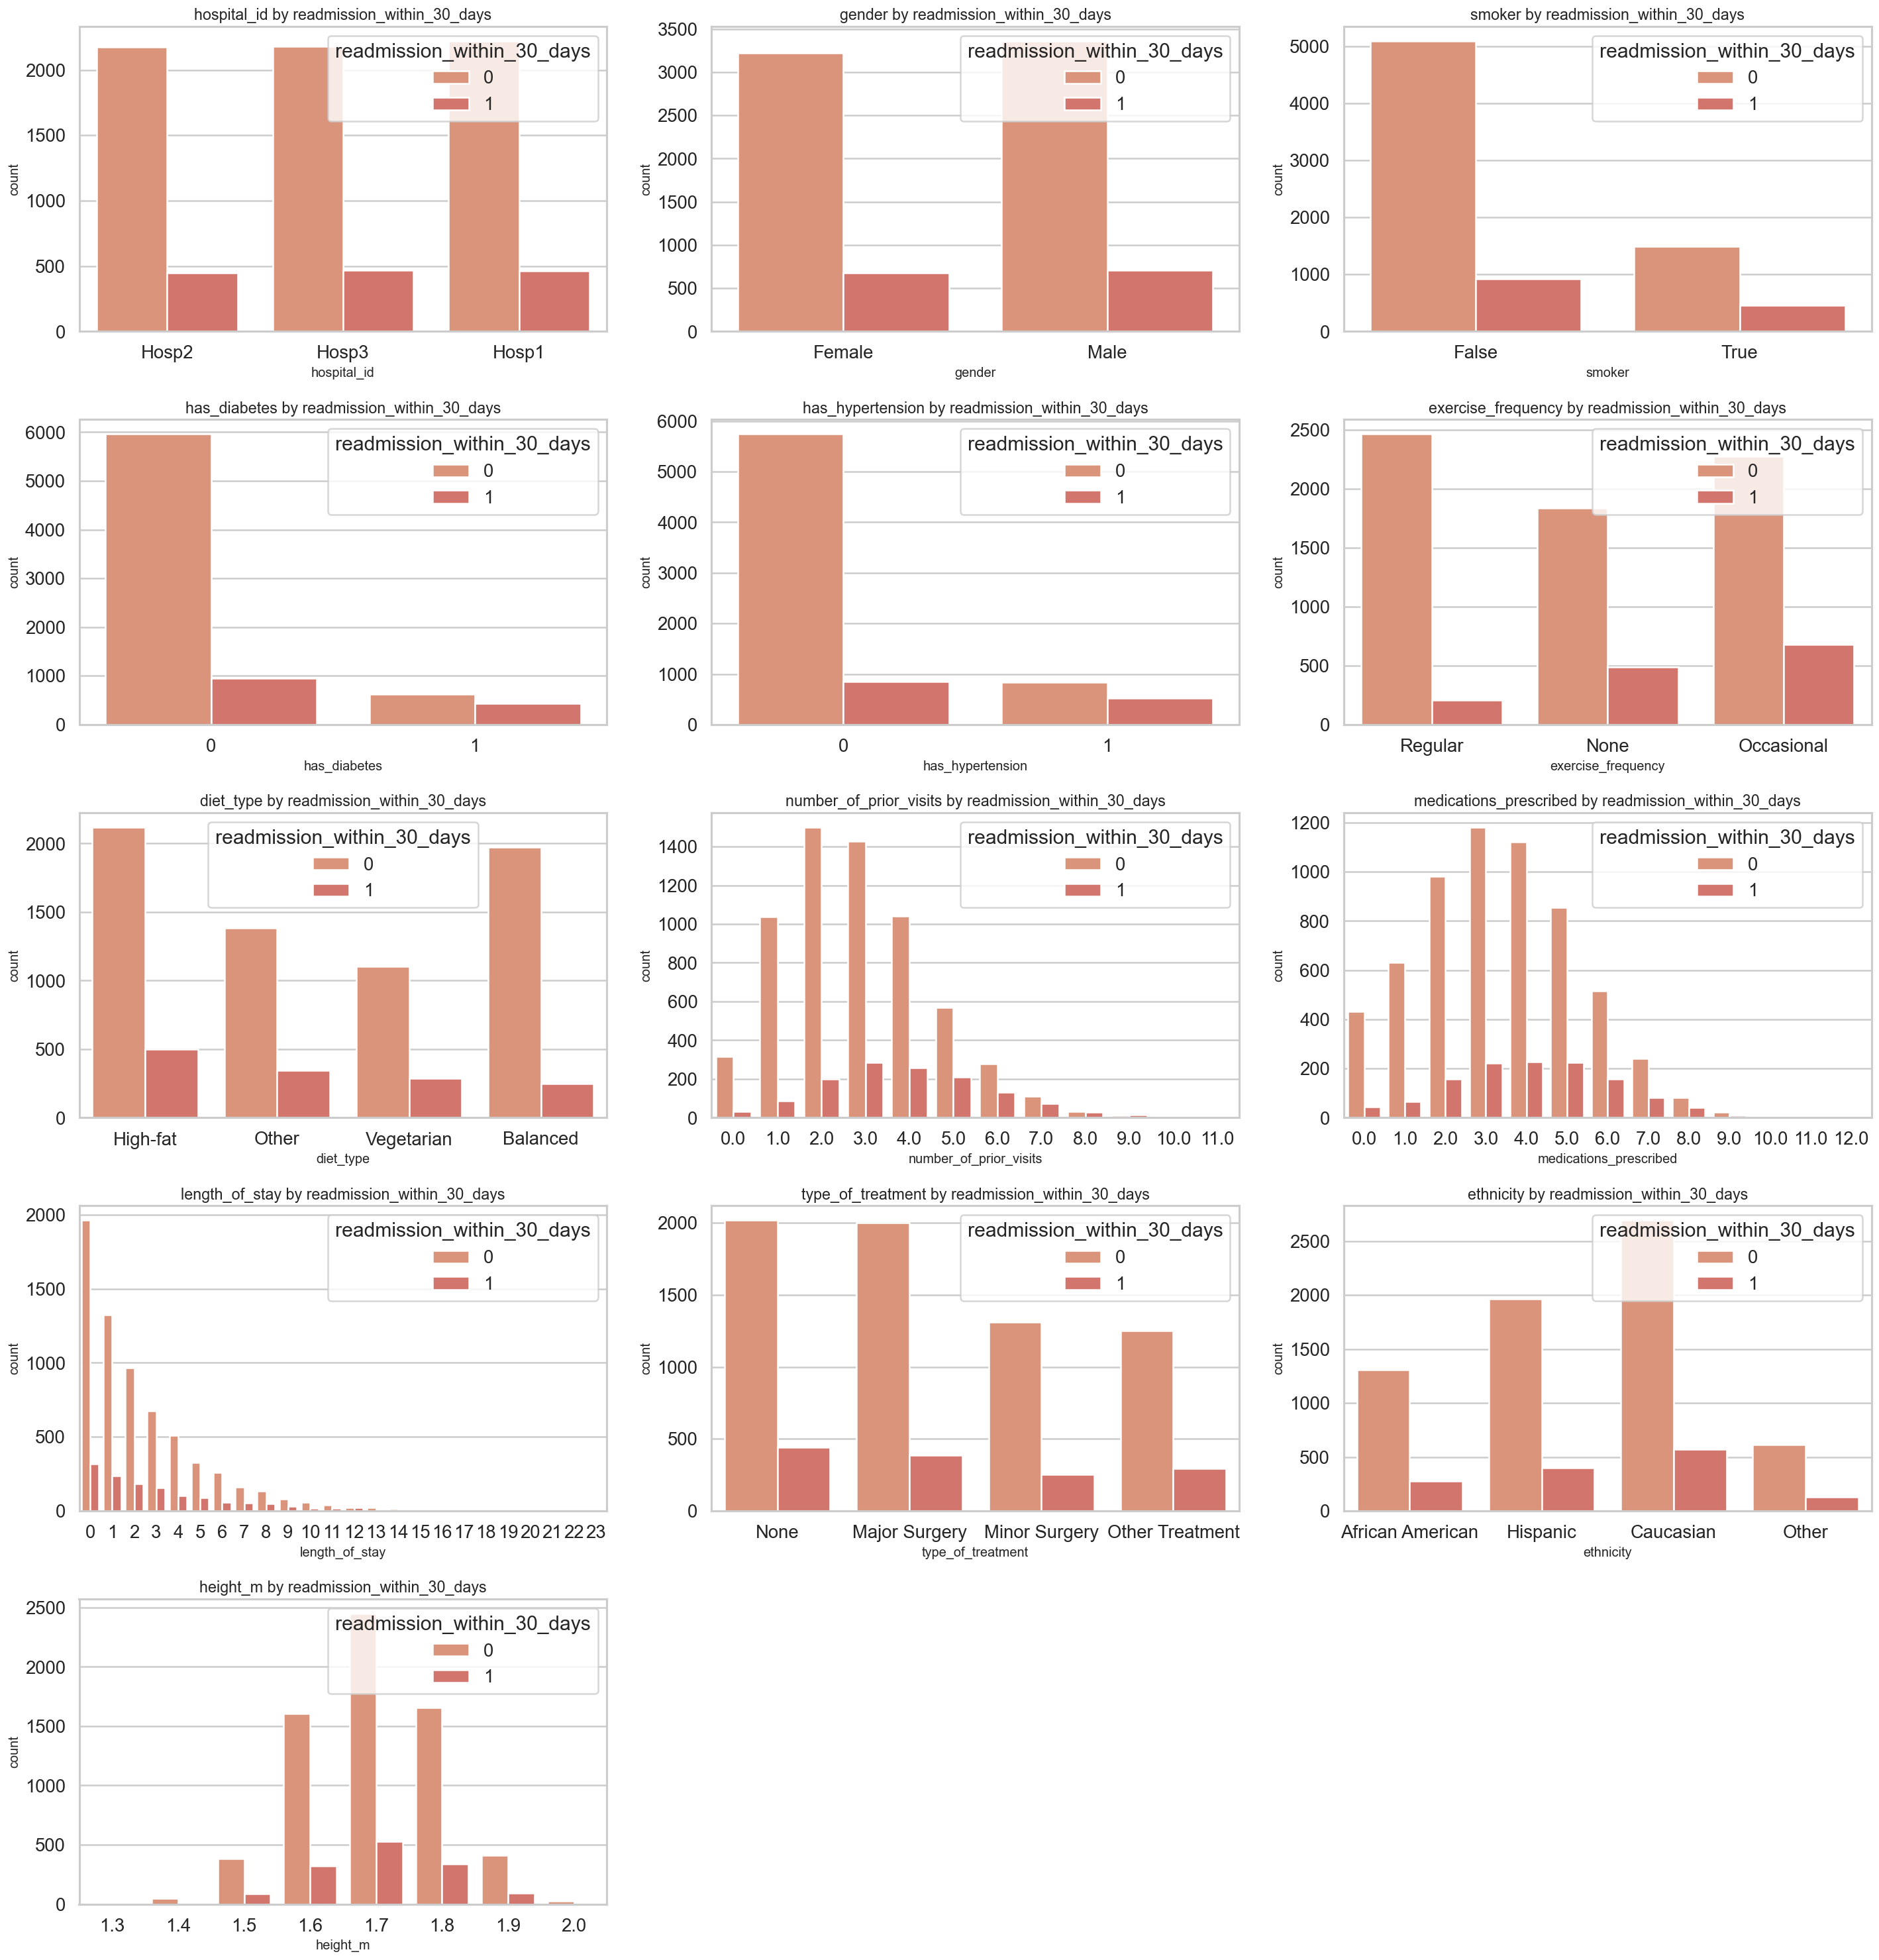
\includegraphics[width=0.75\textwidth]{categories_vs_output_bars.png}
  \caption{Categories vs.\ Readmission Bar Charts}
  \label{fig:categories_vs_output_bars}
\end{figure}

Individual charts can be found in \nameref{sec:appendix-a}. Across most, the ratio of readmissions to non-readmissions is fairly consistent,
however the features like \texttt{Smoker} and \texttt{Has Diabetes} have a higher proportion of positive readmissions when the feature is present
(i.e.\ smoker vs.\ non-smoker, has diabetes vs.\ does not have diabetes). Based off of limited domain knowledge this makes sense, mostly it is
just something to be aware of when considering feature importance.
\subsubsection{Measures}
\begin{figure}[H]
  \centering
  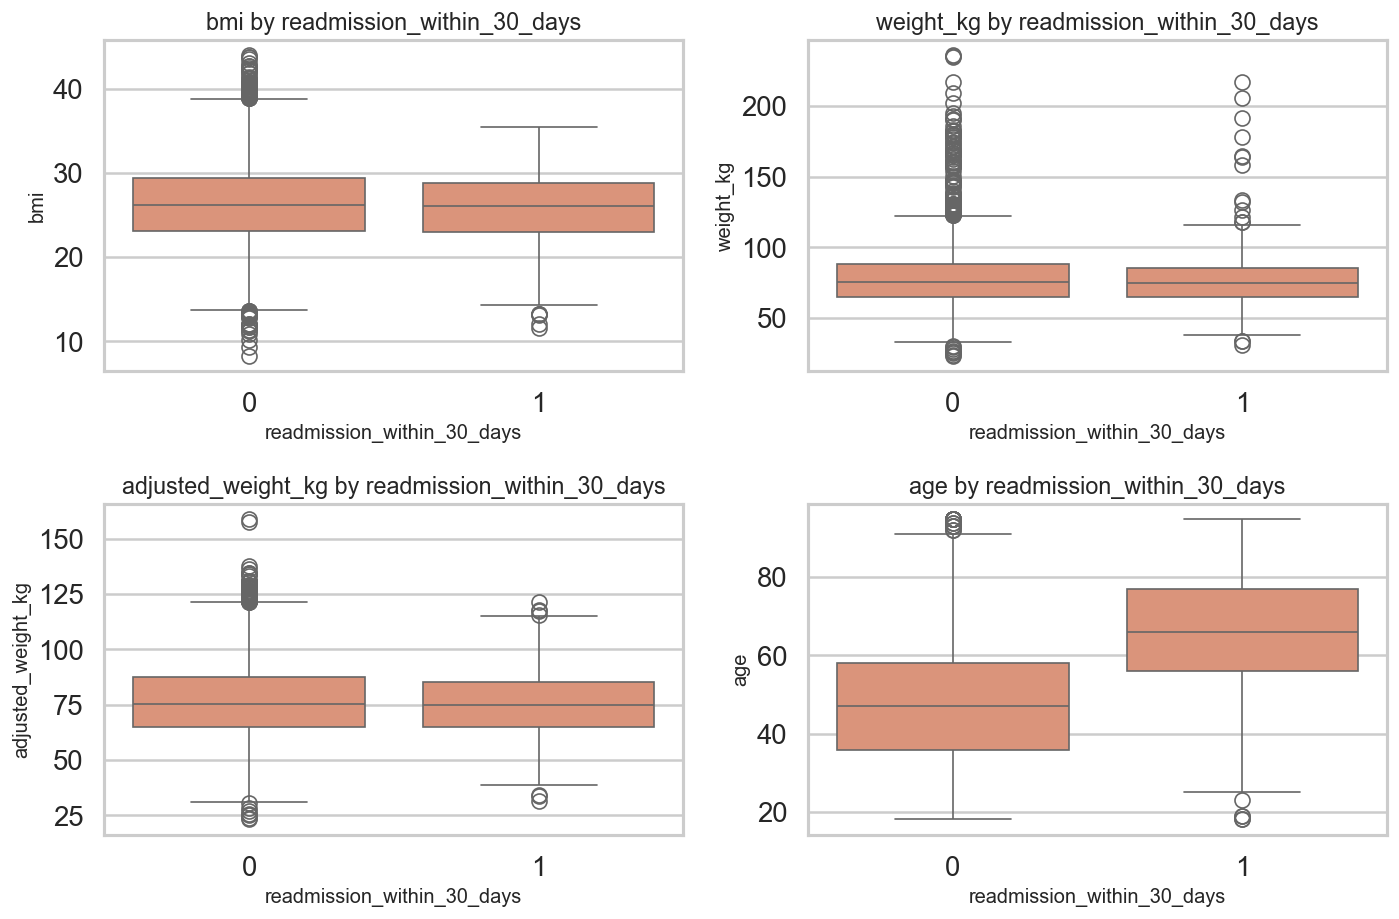
\includegraphics[width=\textwidth]{measures_vs_output_box.png}
  \caption{Measures vs.\ Readmission Box Plots}
  \label{fig:measures_vs_output_boxplots}
\end{figure}

The most noticable distribution difference comes in age, with those who are readmitted
being older on average than those who are not. This seems pretty intuitive, and there
is not much to say about the others

\newpage
\begin{samepage}

  \subsection{Feature Correlations}
  Categorical features were one-hot encoded in order to include the entire dataset in the matrix.

  \begin{figure}[H]
    \centering
    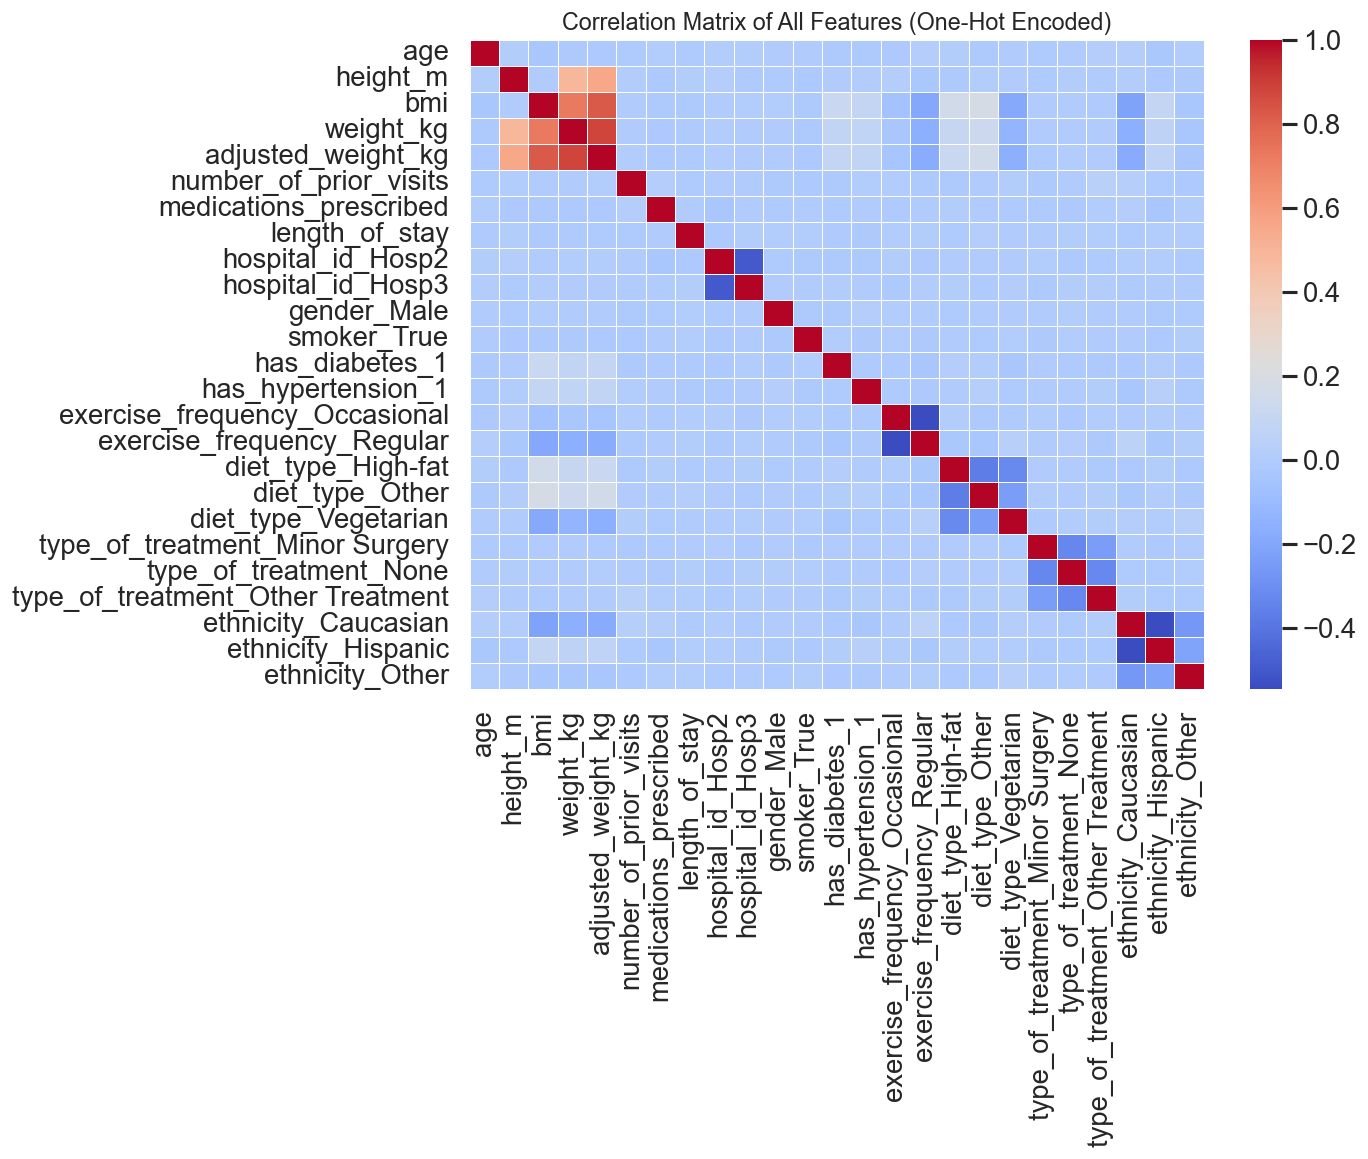
\includegraphics[width=\textwidth]{ohe_corr_matrix.png}
    \caption{Correlation Matrix}
    \label{fig:correlation_matrix}
  \end{figure}
\end{samepage}
\begin{appendices}

  \section{Individual Category vs.~Readmission Charts}
  \label{sec:appendix-a}

  \begin{figure}[H]
    \centering
    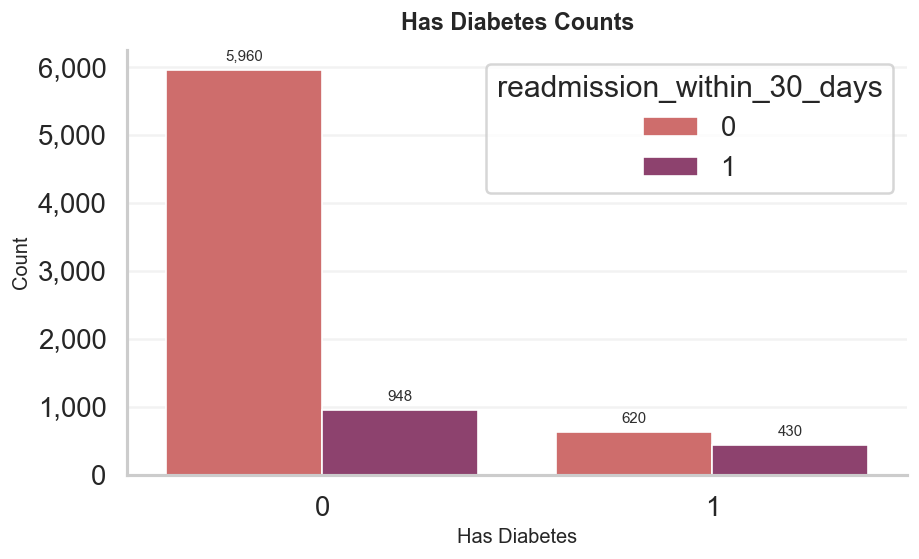
\includegraphics[width=\textwidth]{d_v_o.png}
    \caption{Diabetes vs.\ Readmission}
    \label{fig:diabetes_vs_read}
  \end{figure}

  \begin{figure}[H]
    \centering
    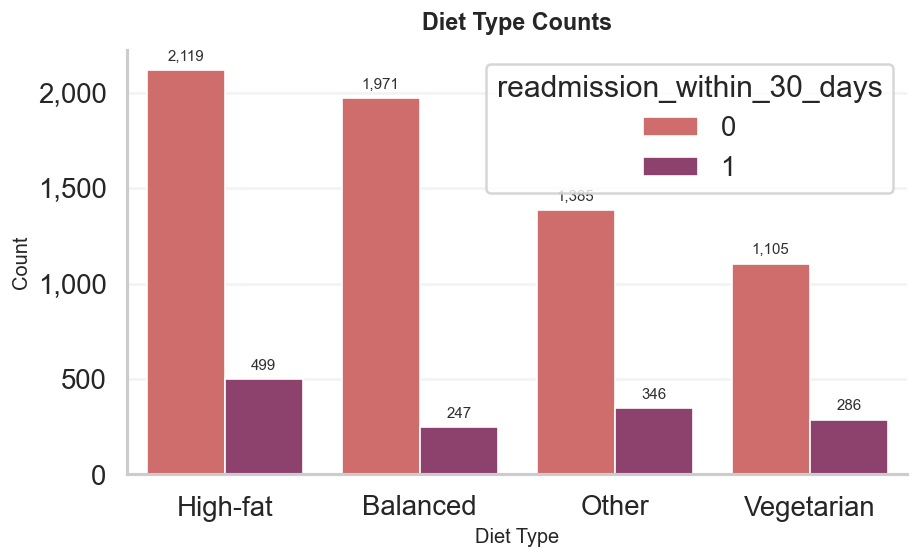
\includegraphics[width=\textwidth]{di_v_o.png}
    \caption{Diet vs.\ Readmission}
    \label{fig:diet_vs_read}
  \end{figure}

  \begin{figure}[H]
    \centering
    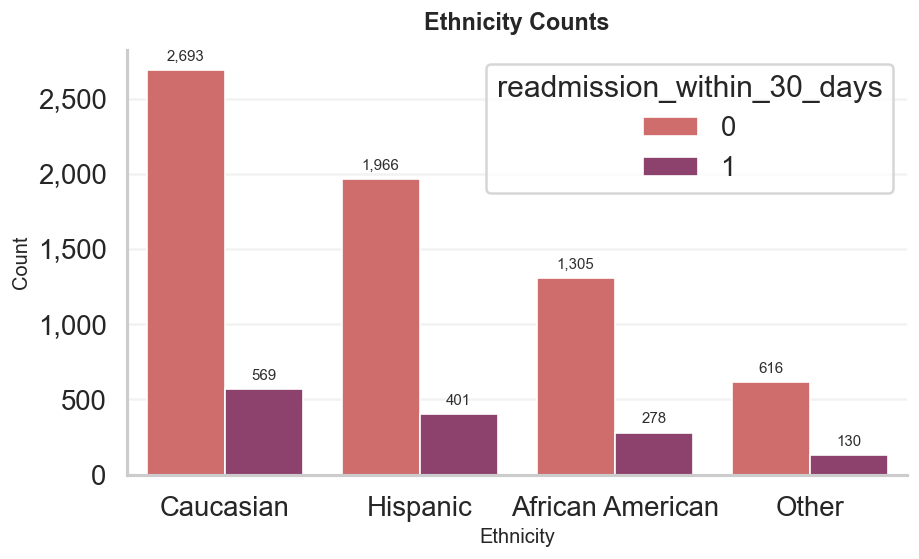
\includegraphics[width=\textwidth]{eth_v_o.png}
    \caption{Ethnicity vs.\ Readmission}
    \label{fig:ethnicity_vs_read}
  \end{figure}

  \begin{figure}[H]
    \centering
    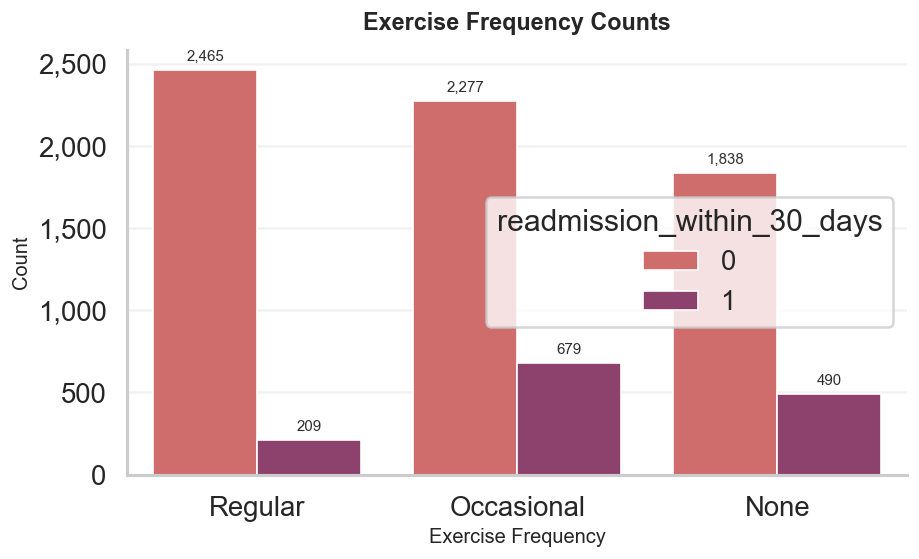
\includegraphics[width=\textwidth]{ex_v_o.png}
    \caption{Exercise vs.\ Readmission}
    \label{fig:exercise_vs_read}
  \end{figure}

  \begin{figure}[H]
    \centering
    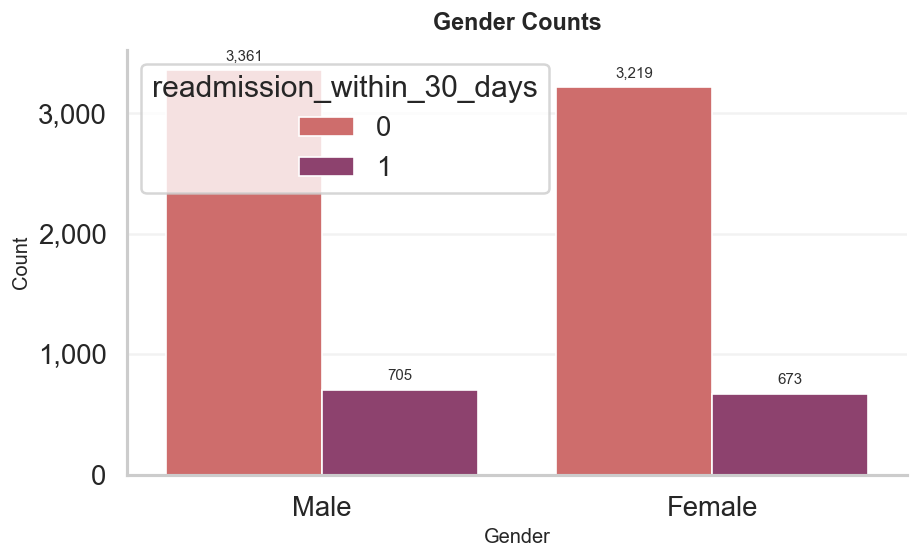
\includegraphics[width=\textwidth]{g_v_o.png}
    \caption{Gender vs.\ Readmission}
    \label{fig:gender_vs_read}
  \end{figure}

  \begin{figure}[H]
    \centering
    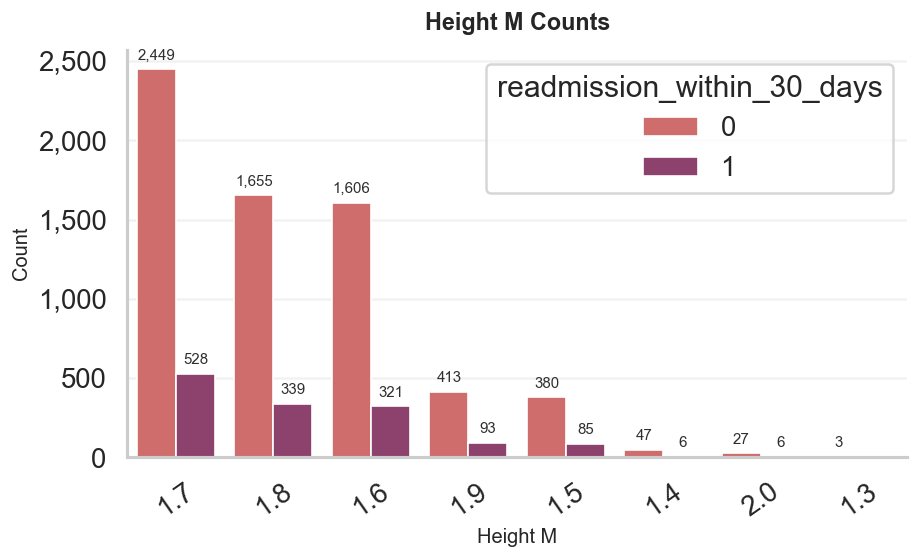
\includegraphics[width=\textwidth]{hei_v_o.png}
    \caption{Height vs.\ Readmission}
    \label{fig:height_vs_read}
  \end{figure}

  \begin{figure}[H]
    \centering
    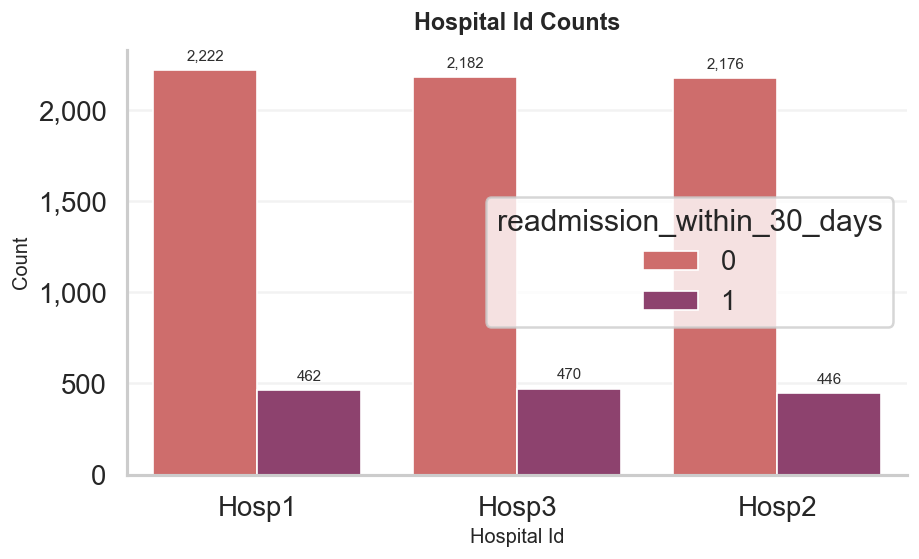
\includegraphics[width=\textwidth]{hid_v_out.png}
    \caption{Hospital ID vs.\ Readmission}
    \label{fig:hospital_id_vs_read}
  \end{figure}

  \begin{figure}[H]
    \centering
    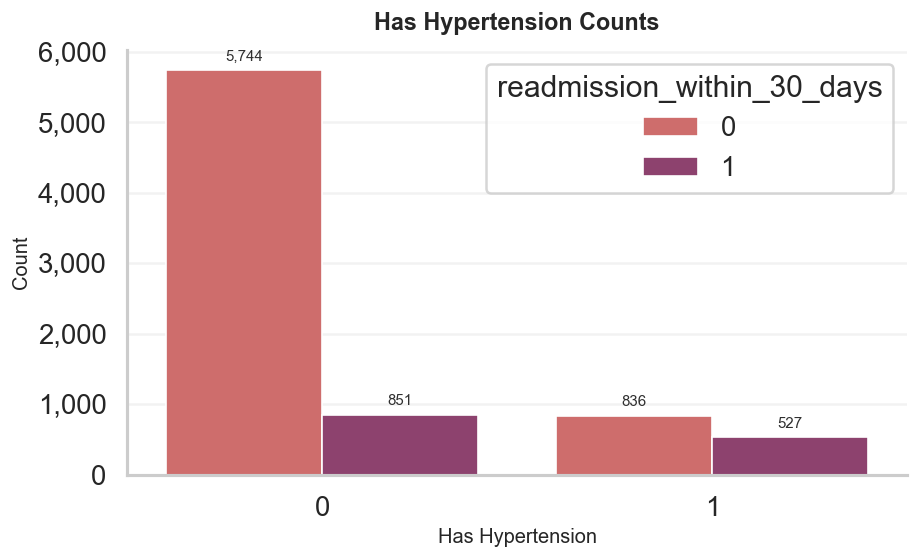
\includegraphics[width=\textwidth]{ht_v_o.png}
    \caption{Hypertension vs.\ Readmission}
    \label{fig:hypertension_vs_read}
  \end{figure}

  \begin{figure}[H]
    \centering
    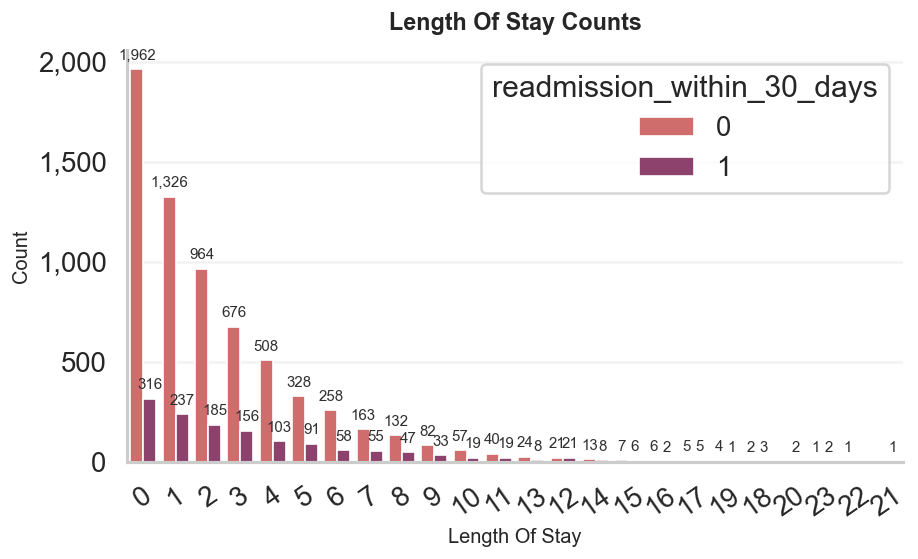
\includegraphics[width=\textwidth]{los_v_o.png}
    \caption{Length of Stay vs.\ Readmission}
    \label{fig:length_of_stay_vs_read}
  \end{figure}

  \begin{figure}[H]
    \centering
    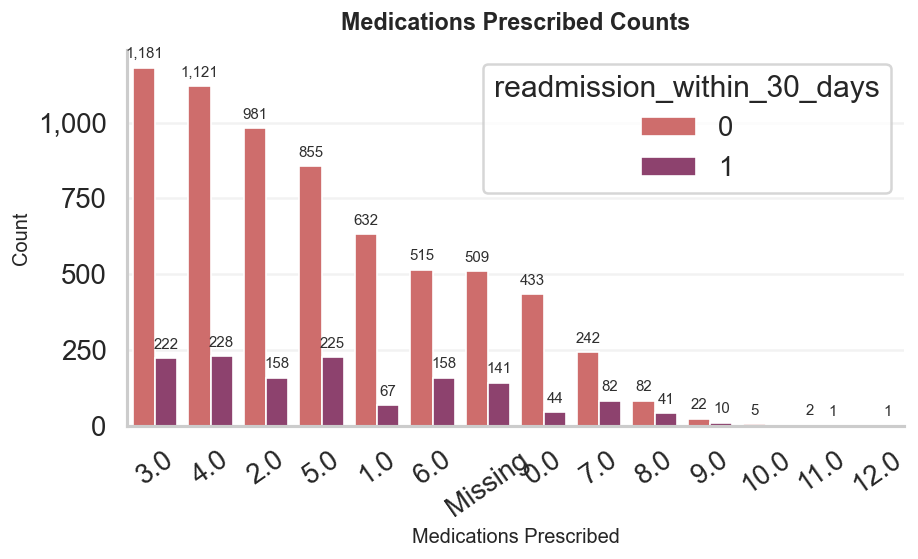
\includegraphics[width=\textwidth]{med_v_o.png}
    \caption{Num Medications vs.\ Readmission}
    \label{fig:num_medications_vs_read}
  \end{figure}

  \begin{figure}[H]
    \centering
    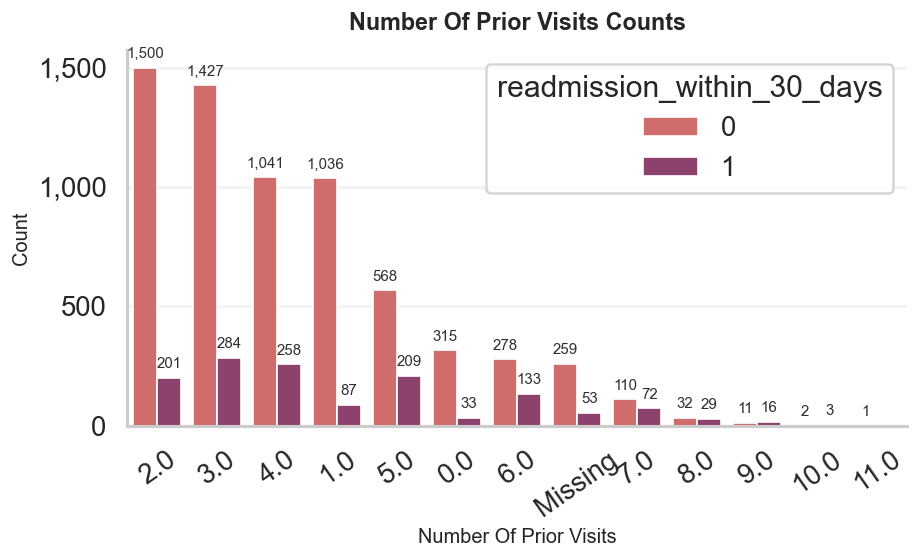
\includegraphics[width=\textwidth]{nm_v_o.png}
    \caption{Num Prior Visits vs.\ Readmission}
    \label{fig:num_prior_visits_vs_read}
  \end{figure}

  \begin{figure}[H]
    \centering
    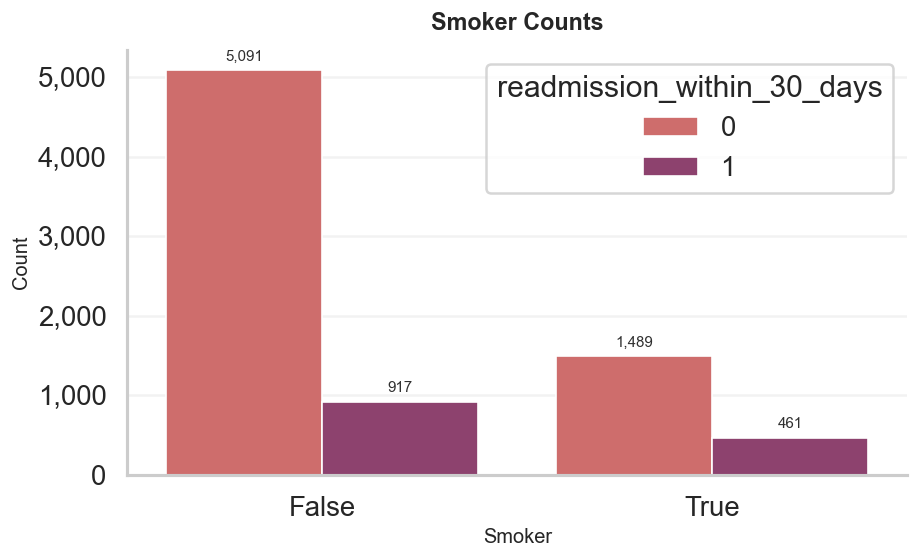
\includegraphics[width=\textwidth]{s_v_o.png}
    \caption{Smoker vs.\ Readmission}
    \label{fig:smoker_vs_read}
  \end{figure}

  \begin{figure}[H]
    \centering
    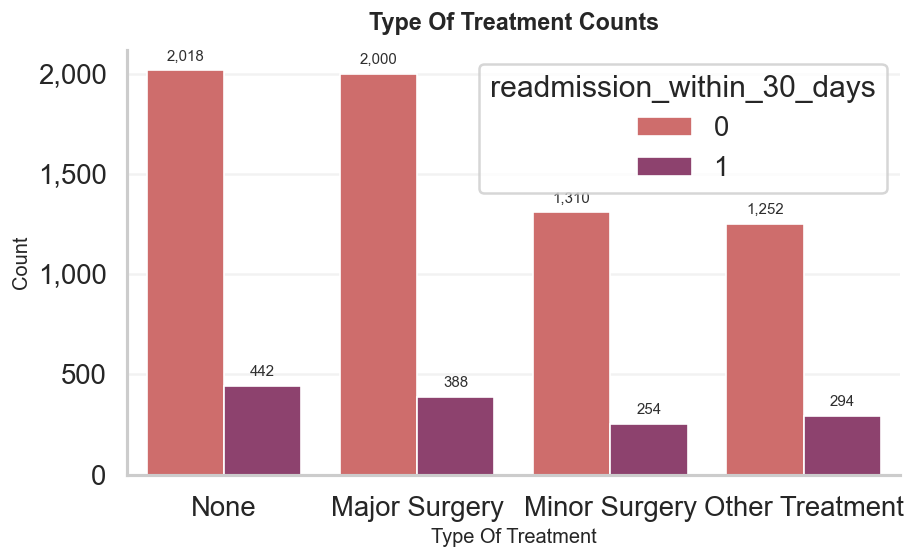
\includegraphics[width=\textwidth]{tot_v_o.png}
    \caption{Type of Treatment vs.\ Readmission}
    \label{fig:type_of_treatment_vs_read}
  \end{figure}

\end{appendices}

\end{document}